\documentclass{standalone}
\usepackage{tikz}
\begin{document}
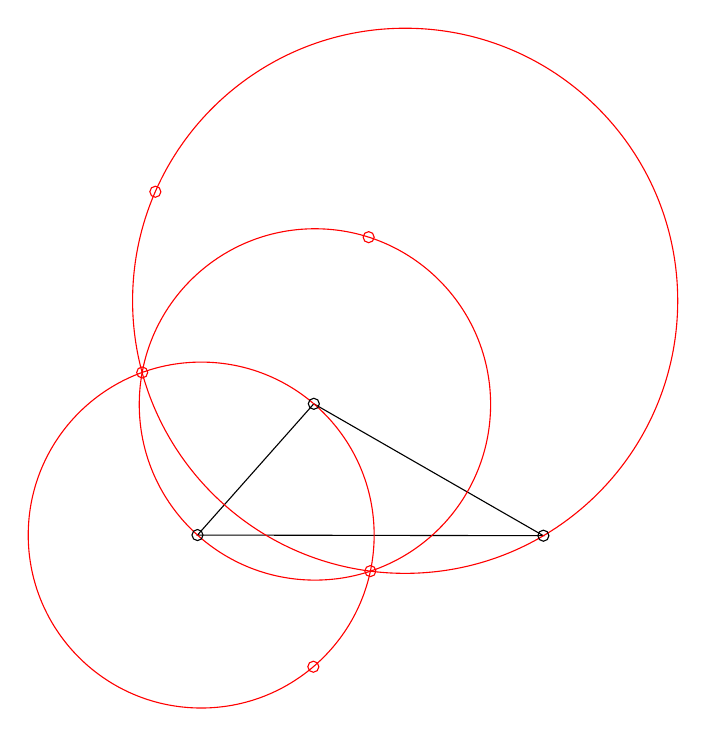
\begin{tikzpicture}[x=1pt,y=1pt]
\draw (229.94,-197.39) -- (104.95,-197.16) -- (146.99,-149.73) -- cycle;
\draw[red] (106.29,-197.16) circle (62.50);
\draw[red] (179.99,-112.51) circle (98.49);
\draw[red] (147.39,-149.96) circle (63.48);
\draw[red] (146.82,-244.74) circle (2.00);
\draw[red] (89.73,-73.10) circle (2.00);
\draw[red] (166.80,-89.52) circle (2.00);
\draw (146.99,-149.73) circle (2.00);
\draw (229.94,-197.39) circle (2.00);
\draw (104.95,-197.16) circle (2.00);
\draw[red] (167.42,-210.19) circle (2.00);
\draw[red] (84.97,-138.41) circle (2.00);
\end{tikzpicture}
\end{document}
